\documentclass[10pt,a4paper]{article}
\usepackage[utf8]{inputenc}
\usepackage[spanish]{babel}
\usepackage{amsmath}
\usepackage{amsfonts}
\usepackage{amssymb}
\usepackage{graphics}
\usepackage{graphicx}
\usepackage{xcolor}
\usepackage{listings}
\usepackage{csvsimple}
\usepackage{caption}
\usepackage[left=2cm,right=2cm,top=2cm,bottom=2cm]{geometry}

\renewcommand*\contentsname{Índice} %Nombre del indice

\begin{document}
\lstset{language=C++,
	basicstyle=\footnotesize,
	extendedchars=true,
	literate={á}{{\'a}}1 {ã}{{\~a}}1 {é}{{\'e}}1 {ú}{{\'u}}1 {ó}{{\'o}}1,
	backgroundcolor=\color{black!5}
	}
	
\begin{titlepage}
	\centering
	{
\includegraphics[scale=0.5]{Logo_UGR.png}\par}
	\vspace{1cm}
	{\bfseries\Large Escuela T\'ecnica Superior de Ingeniería Informática y Telecomunicaciones \par}
	\vspace{2.5cm}
	{\scshape\Huge Pr\'actica 1: An\'alisis de eficiencia de algoritmos \par}
	\vspace{3cm}
	{\itshape\Large Doble Grado Ingeniería Informática y Matemáticas}
	\vfill
	{\Large Autores: \par}
	{\Large Jose Alberto Hoces Castro\par}
	{\Large Javier Gómez López \par}
	{\Large Moya Mart\'in Castaño \par}
	\vfill
	{\Large Marzo 2022 \par}
\end{titlepage}

\thispagestyle{empty}
\null
\vfill

%%Información sobre la licencia
\parbox[t]{\textwidth}{
  
\includegraphics[scale=0.05]{by-nc-sa.png}\\[4pt]
  \raggedright % Texto alineado a la izquierda
  \sffamily\large
  {\Large Este trabajo se distribuye bajo una licencia CC BY-NC-SA 4.0.}\\[4pt]
  Eres libre de distribuir y adaptar el material siempre que reconozcas a los\\
  autores originales del documento, no lo utilices para fines comerciales\\
  y lo distribuyas bajo la misma licencia.\\[4pt]
  \texttt{creativecommons.org/licenses/by-nc-sa/4.0/}
}

\newpage

\tableofcontents

\newpage
\section{Introducción}

Esta primera práctica, \textbf{Práctica 1}, consiste en el análisis de eficiencia de algoritmos, consiste en tres partes distintas:
\begin{itemize}
	\item \textbf{Análisis de la eficiencia teórica:} estudio de la complejidad teórica del algoritmos (Mejor caso, peor caso y caso promedio).
	\item \textbf{Análisis de la eficiencia empírica:} ejecución y medición de tiempos de ejecución de los algoritmos estudiados.
	\item \textbf{Análisis de la eficiencia híbrida:} obtención de las constantes ocultas
\end{itemize}

A continuación, se explican en más profundidad dichas partes.

\subsection{Análisis de la eficiencia teórica}

El análisis de la \textbf{eficiencia teórica} consiste en analizar el tiempo de ejecución de los algoritmos dados para encontrar el peor de los casos, es decir, en qué clase de funciones en notación \(\mathcal{O}\) grande se encuentran. Para ello, hemos utilizado las técnicas de análisis de algoritmos vistas en clase y en la asignatura \textit{Estructura de Computadores}.

\subsection{Análisis de la eficiencia empírica}

Para el análisis de la \textbf{eficiencia empírica}, hemos ejecutado los algortimos en cada uno de nuestros equipos bajo las mismas normas y condiciones, hemos medido el tiempo de ejecución de dichos algoritmos con la biblioteca \texttt{<chrono>}, basándonos en la siguiente estructura del código:

\begin{lstlisting}
#include <chrono>
...

high_resolution_clock::time_point tantes, tdespues;
duration <double> transcurrido;
..

tantes = high_resolution_clock::now();
//Sentencia o programa a medir
tdepues = high_resolution_clock::now();
transcurrido = duration_cast<duration<double>>(tdespues-tantes);
\end{lstlisting}

Además, para automatizar el proceso de ejecución de los algortimos, hemos usado la siguiente estrucutra para generar nuestros scripts:
\begin{lstlisting}[language=bash]
i = #valor de la primera iteracion

while [ $i -le #valor ultima iteracion ]
do
./programa_a_ejecutar $i >> salida.dat
i=$[i+#salto entre valores para conseguir 26 puntos]
done
\end{lstlisting}

Hemos ejecutado cada algoritmo 15 veces en cada uno de los tamaños que han sido probados, y hemos hecho la media de ellos para reducir perturbaciones que puedan ocurrir de manera aleatoria y que nos lleven al mejor o peor caso, obteniendo de esta forma casos promedio. 

Cabe destacar que para \textit{seleccion} e \textit{insercion} hemos además ejecutado dos programas adicionales para obtener el mejor y peor caso de estos, pero este hecho lo detallaremos más adelante. \\

\subsection{Análisis de la eficiencia híbrida}
Para el análisi de la eficiencia híbrida, hemos tomado los datos de cada uno de los alumnos del grupo y hemos hallado la \(K\)(constante oculta). Para ello, hemos usado gnuplot. \\

Lo primero que hacemos es definar la función a la que queremos ajustar los datos. Tenemos que tener en cuenta el análisis teórico que hemos realizado previamente para saber cuál va a ser la forma de esta función. Podemos definir esta función en gnuplot mediante el siguiente comando (ejemplo para \(\mathcal{O}(n^2)\)):
\begin{lstlisting}[language=bash]
gnuplot> f(x) = a0*x*x+a1*x+a2
\end{lstlisting}

El siguiente paso es indicarle a gnuplot que haga la regresión:
\begin{lstlisting}
gnuplot> fit f(x) 'salida.dat' via a0,a1,a2
\end{lstlisting}
donde \texttt{'salida.dat'} es nuestro dataset. 

La parte que más nos interesa es la parte donde pone \texttt{Final set of parameters}, pues ahí están nuestros coeficientes.

\section{Desarrollo}

A continuación, realizaremos el estudio individual de cada algortimo, como se ha descrito anteriormente.

\subsection{Inserción}
\subsection{Selección}
\subsection{Quicksort}
\subsection{Heapsort}
\subsection{Floyd}
\lstinputlisting[language=Python]{./Codes/floyd.cpp}

\subsubsection{Eficiencia teórica}

Como podemos observar en los comentarios del código que hemos hecho en la función \texttt{void Floyd}, estamos ante una función que pertenece a \(\mathcal{O}(n^3)\). Son tres bucles \texttt{for} que están anidados, cada uno \(\mathcal{O}(n)\), por tanto, multiplicando los órdenes obtenemos que la función es \(\mathcal{O}(n^3)\), es decir,
\[
	T(n) \in \mathcal{O}(n^3)
\]
donde \(T(n)\) es la función que expresa el tiempo de ejecución del algoritmo.

\subsubsection{Eficiencia empírica}

Tras ejecutar el algoritmo en un rango de 176 a 2000 elementos, con saltos de 76 unidades por ejecución, obtenemos los siguientes resultados:

\begin{table}[h!]
	\centering
	\footnotesize
	\scalebox{0.75}{
		\begin{tabular}{|c|c|}
			\hline
			\multicolumn{2}{|c|}{\textsf{Intel Core i7-6700 3.40 GHz}}
			\\\hline
			\bfseries Elementos (n) & \bfseries Tiempo (s)
			\csvreader{./data/Javi5454/salida_floyd.csv}{}
			{\\\hline\csvcoli&\csvcolii}
			\\\hline
		\end{tabular}
		}
		\hspace{2cm}
		\scalebox{0.75}{
		\begin{tabular}{|c|c|}
			\hline
			\multicolumn{2}{|c|}{\textsf{Ordenador Jota}}
			\\\hline
			\bfseries Elementos (n) & \bfseries Tiempo (s)
			\csvreader{./data/Jota/salida_floyd.csv}{}
			{\\\hline\csvcoli&\csvcolii}
			\\\hline
			\end{tabular}
			}
		\hspace{2cm}
		\scalebox{0.75}{
		\begin{tabular}{|c|c|}
			\hline
			\multicolumn{2}{|c|}{\textsf{Ordenador Moya}}
			\\\hline
			\bfseries Elementos (n) & \bfseries Tiempo (s)
			\csvreader{./data/Moya/salida_floyd.csv}{}
			{\\\hline\csvcoli&\csvcolii}
			\\\hline
		\end{tabular}
		}
		\caption{Experiencia empírica de algoritmo de Floyd sin optimizar}
\end{table}

Observamos pequeñas diferencias, pero en general nada fuera de lo común. Estas diferencias son debidas a los distintos agentes tecnológicos usados para la realización del análisis de la eficiencia empírica en esta práctica.

\subsubsection{Eficiencia híbrida}

A través de la eficiencia híbrida, comprobaremos que el ajuste teórico realizado es correcto. Para realizar este análisi, tomamos los datasets de todos los integrantes del grupo. \\

\begin{figure}[h!]
\centering
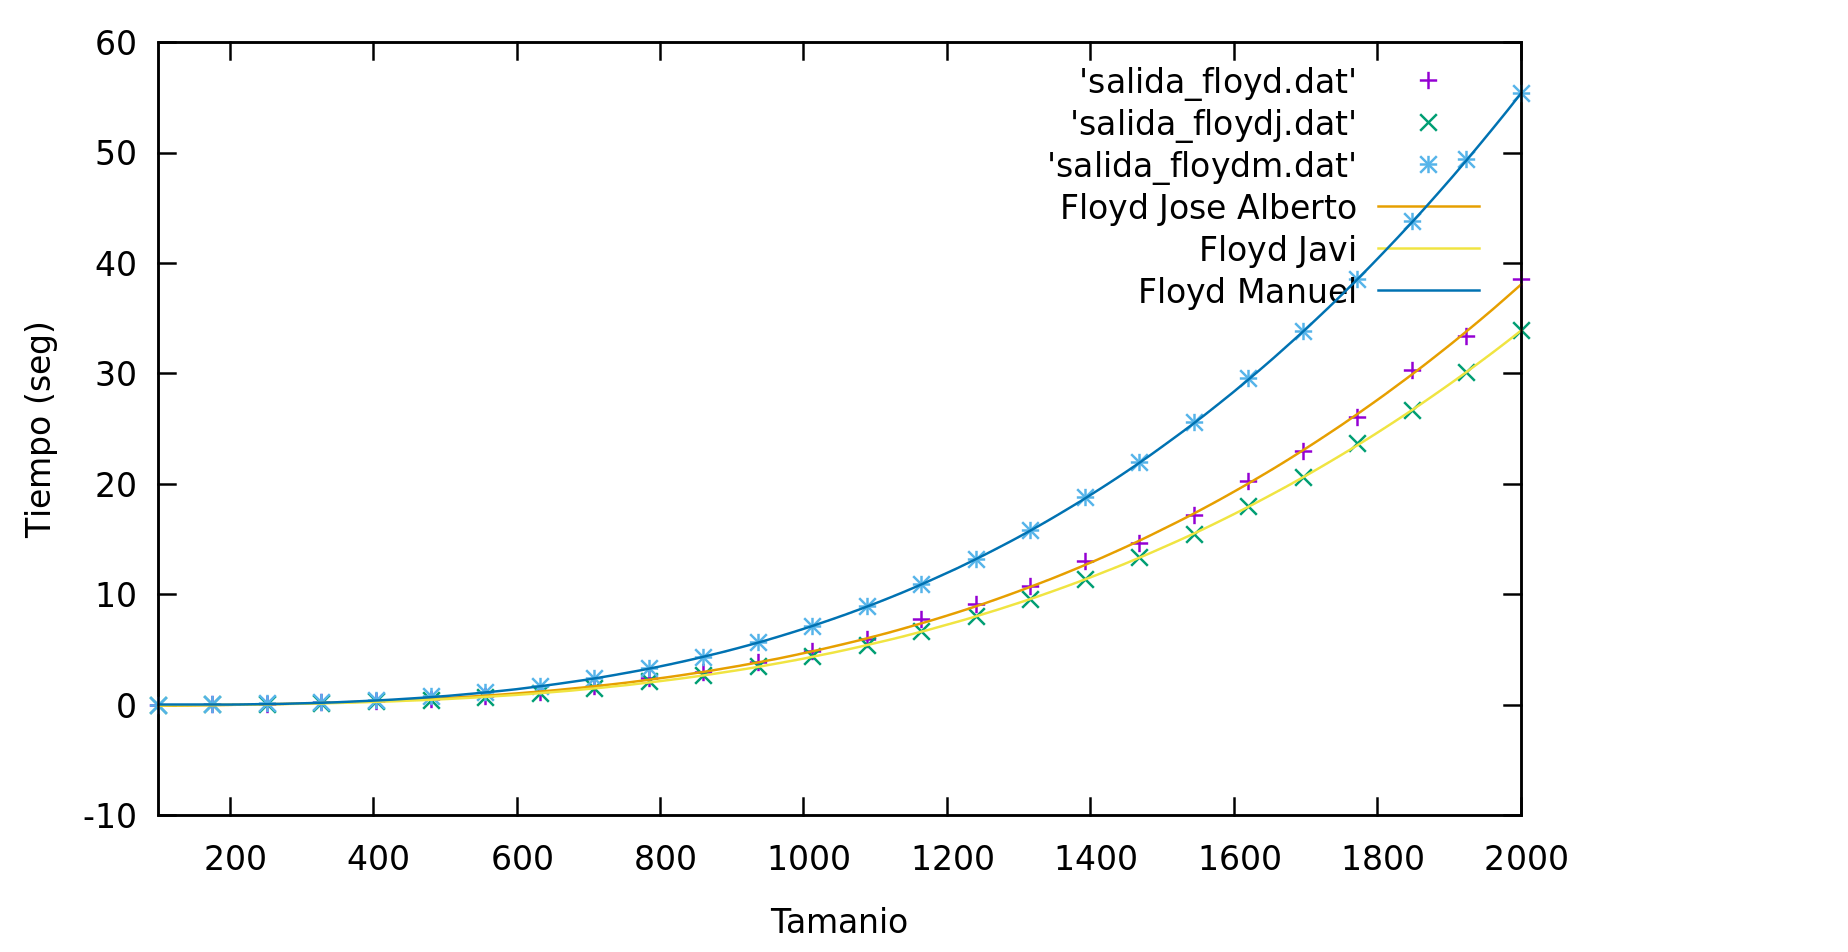
\includegraphics[scale=0.15]{../../Images/floyd_combinados.png}
\caption{Gráfica con los tiempos de ejecución del \\algoritmo de Floyd}
\end{figure}

En esta gráfica están representados los 26 puntos obtenidos tras la ejecución del algoritmo de Floyd en los distintos equipos de los integrantes equipos. Tras una serie de cálculos con gnuplot, observamos que las constantes ocultas son:
\begin{itemize}
	\item i7-6700 3.40Ghz \(\rightarrow T_1(n) = 4.38237 \cdot 10^{-9} x^3 -4.33753 \cdot 10^{-7} x^2 + 0.000337001 x -0.0504332\).
	\item Ordenador Jota \(\rightarrow T_2(n) = 5.12922 \cdot 10^{-9} x^3 -1.11315 \cdot 10^{-6} x^2 + 0.00083571 x - 0.134397\).
	\item Ordenador Moya \(\rightarrow T_3(n) = 6.77297 \cdot 10^{-9} x^3 + 5.13099 \cdot 10^{-7} - 0.000427834 x + 0.0714028\).
\end{itemize} 

A continuación, mostramos una gráfica que muestra otras posibilidades de ajuste para otros puntos, y se observa que el ajuste con una función cúbica es el mejor, confirmando así nuestro análisis teórico. 

\begin{figure}[h!]
\centering
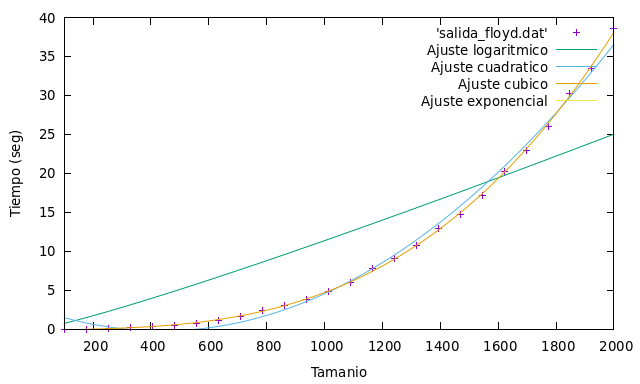
\includegraphics[scale=0.4]{../../Images/floy_comparacion.png}
\caption{Bondad de ajuste cúbico Floyd}
\end{figure}

Podemos observar que nuestro análisis teórico es correcto. Además, podemos observarlo con el coeficiente de regresión para cada una de nuestra funciones de ajuste:
\begin{itemize}
	\item \(T_1(n) \longrightarrow R^2 = 0.00204522\)
	\item \(T_2(n) \longrightarrow R^2 = 0.044778\)
	\item \(T_3(n) \longrightarrow R^2 = 0.000855184\)
\end{itemize}

Estos valores son muy cercanos a 0, y por tanto indican que el ajuste es muy bueno.
\subsection{Hanoi}

\end{document}